%%%%%%%%%%%%%%%%%%%%%%%%%%%%%%%%%%%%%%%%%%%%%%%%%%%%%%%%%%%%%%%%
\section{Higgs Mechanism}

%There are four forces in nature, gravity, electromagneticism, weak force 
%and strong force. Gravity is described by general relativity. 
Properties of elementary particles in nature and their interactions (forces)
to each other are described by Standard Model (SM) in particle physics. It is 
based on gauge symmetry and the group sturucture, 
$SU(3)_c \times SU(2)_L \times U(1)_Y$, where  $SU(3)_c$, $SU(2)_L$, and $U(1)_Y$  
describe color, weak isospin, and hyper charge, respectively. 
The gauge symmetry requires the weak gauge bosons to be massless,
but we know that Weak gauge bosons, $W^\pm$ and $Z$ are massive. 
The cure for this is the Higgs mechanism which breaks $SU(2)_L \times U(1)_Y$
to $U(1)_{EM}$, thus giving mass to weak bosons but keeping photons massless. 

\subsection{How particles become massive : Higgs Mechanism}
Since EW theory is based on $SU(2)$ symmetry, the Higgs field is 
given as a $SU(2)$ doublet, 
\begin{eqnarray} 
\phi = \left(  \begin{array}{c} \phi^+ \\ \phi^0 \end{array} \right)
\end{eqnarray} 
where each element is a complex field, 
\begin{eqnarray} 
\phi^+ = \frac{\phi_1 + i\phi_2}{\sqrt{2}} 
\qquad \textrm{ and } \qquad  
\phi^0 = \frac{\phi_3 + i\phi_4}{\sqrt{2}}.
\end{eqnarray} 
We start with the Higgs Lagrangian to understand the essence of SSB 
before making the things more complicated. The full SM Lagrangian will be discussed after that.  
The Higgs Lagrangian is composed of kinetic and potential terms. 
\begin{eqnarray} 
\mathcal{L}_\phi 
=
\underbrace{
    \left( \partial_\mu \phi \right)^\dagger \left( \partial^\mu \phi \right)
}_\text{kinetic term} 
- 
\underbrace{
    \left( \mu^2 \phi^\dagger \phi + \lambda \left( \phi^\dagger \phi \right)^2 \right)
}_\text{potential} 
\end{eqnarray} 
where $\mu^2<0$ and $\lambda>0$.
The potential $V\left( \phi^\dagger \phi \right)$ is invariant under 
$SU(2)$ local gauge transformation, 
\begin{eqnarray} 
\phi(x) 
\rightarrow 
\phi(x)' = e^{i \vec{\alpha}(x) \cdot \frac{\vec{\sigma}}{2}} \phi(x)
\end{eqnarray} 
where $\vec{\alpha}(x)$ is a vector of parameters and  
$\vec{\sigma}$ is a vector of Pauli matrices. 
$V\left( \phi^\dagger \phi \right)$ has the minimum at 
$\displaystyle  \phi^\dagger \phi = -\frac{\mu^2}{2\lambda} = \frac{v^2}{2}$ where 
$v$ is the vacuum expectation value of the Higgs field $\phi$.
Due to the SU(2) symmetry the choice of vacuum state is not definite 
as seen in the following equation, 
\begin{eqnarray} 
\phi^\dagger \phi = \frac{1}{2} \left( \phi_1^2 + \phi_2^2 + \phi_3^2 + \phi_4^2\right) 
\end{eqnarray} 
This leads to an appropriate choice of vacuum for the physics of interest. 
We choose the vacuum state, $\phi_0$
\begin{eqnarray} 
\phi_0 = \frac{1}{\sqrt{2}} \left(  \begin{array}{c} 0 \\ v \end{array} \right)
\end{eqnarray} 
and expand around it by $H(x)$
\begin{eqnarray} 
\phi(x) = \frac{1}{\sqrt{2}} \left(  \begin{array}{c} 0 \\ v + H(x) \end{array} \right)
\end{eqnarray} 
where $H(x)$ is the physical Higgs field.  
In order to make the lagrangian invariant under SU(2) transformation,
the derivative $\partial_\mu$ should be replaced by the covariant 
derivative $\mathcal{D}_\mu$
\begin{eqnarray} 
\mathcal{D}_\mu 
= 
\partial_\mu - ig_1 \frac{Y}{2} B_\mu - ig_2 \frac{\vec{\sigma}}{2} \cdot \vec{W}_\mu. 
\end{eqnarray} 
$B_\mu$ and $\vec{W}_\mu$ are the vector field(s) needed for U(1) and 
SU(2) gauge invariance, respectively. 
$g_1$ and $g_2$ are the couplings that decide the strength of 
interactions associated with $B_\mu$ and $\vec{W}_\mu$. 
$Y$(weak hypercharge) and $\frac{\vec{\sigma}}{2}$ are the generators for U(1) and SU(2), respectively. 
Putting this into the Lagrangian $\mathcal{L_\phi}$, the kinetic term becomes 
\begin{eqnarray} 
\left( \mathcal{D}_\mu \phi \right)^\dagger \left( \mathcal{D}^\mu \phi \right) 
&=& ... +  
\phi^\dagger 
\left[ - ig_1 \frac{Y}{2} B^\mu
       - ig_2 \frac{\vec{\sigma}}{2} \cdot \vec{W}^\mu \right]^\dagger 
\left[ - ig_1 \frac{Y}{2} B^\mu
       - ig_2 \frac{\vec{\sigma}}{2} \cdot \vec{W}^\mu \right] 
\phi  
\end{eqnarray}
In order to derive masses of W and Z boson, we use the vacuum state of Higgs field $\phi_0$
because mass are present even without dynamical field.  
With $Y=1$ and $\displaystyle \phi = \frac{1}{\sqrt{2}} \left(  \begin{array}{c} 0 \\ v \end{array} \right)$, 
writing the explicitly in $2\times2$ matrices, 
\begin{eqnarray}
\label{eq:WZmass}
\begin{array}{ccc} \multicolumn{2}{c}{ \displaystyle \vspace{0.3cm}   
\frac{1}{8} \left| \left(  \begin{array}{cc} 
g_1 B_\mu + g_2 W_\mu^3     & g_2 (W_\mu^1 - iW_\mu^2) \\
g_2 (W_\mu^1 + iW_\mu^2)    & g_1 B_\mu - g_2 W_\mu^3 \end{array} \right) 
\left(  \begin{array}{c} 0 \\ v \end{array} \right) \right|^2 
} & \\ & \multicolumn{2}{l}{\hspace{2cm} \vspace{0.3cm} \displaystyle   
= \frac{v^2}{8} \left| \left(  \begin{array}{c} 
g_2 (W_\mu^1 - iW_\mu^2) \\
g_1 B_\mu - g_2 W_\mu^3 
\end{array} \right) \right|^2} \\  
& \multicolumn{2}{l}{\hspace{2cm}  \displaystyle   
=   
\frac{v^2 g_2^2}{8} \left[ \left( W_\mu^1 \right)^2  + \left( W_\mu^2 \right)^2 \right] 
+ \frac{v^2}{8} \left( g_1 B_\mu - g_2 W_\mu^3 \right)^2
} \end{array}    
\end{eqnarray} 
The first term can be written converting $W^1$ and $W^2$ into 
charge states $\displaystyle W^\pm = \frac{1}{\sqrt{2}} \left( W^1 \mp iW^2 \right)$, 
\begin{eqnarray}
\frac{1}{2} \left( \frac{v g_2}{2} \right)^2 
\left[ \left( W_\mu^+ \right)^2  + \left( W_\mu^- \right)^2 \right]. 
\end{eqnarray} 
Thus, we have the mass of charged W boson $\displaystyle M_W = \frac{v g_2}{2}$.
Now we know that the second term in \ref{eq:WZmass} should correspond 
Z boson because that is the only remaining mass boson. Because the 
mixed fields should have the same normalization, the physical field for 
Z boson $Z_\mu$ is 
\begin{eqnarray} 
Z_\mu = \frac{\left( g_1 B_\mu - g_2 W_\mu^3 \right)}{\sqrt{g_1^2+g_2^2}}  
\end{eqnarray} 
which gives its mass $\displaystyle M_Z = \frac{v}{2} \sqrt{g_1^2+g_2^2}$. 
We have an orthogonal field that is massless 
(thus mass term does not appear in the Lagrangian), 
\begin{eqnarray} 
A_\mu = \frac{\left( g_1 B_\mu + g_2 W_\mu^3 \right)}{\sqrt{g_1^2+g_2^2}}  
\end{eqnarray}
This is the field that remains unbroken by SSB. So, it corresponds to photon. 
%Using the definition of weak mixing angle, $\theta_W$, 
%\begin{equation} 
%\sin \theta_W = \frac{g_1}{\sqrt{g_1^2+g_2^2}}, \textrm{ and } 
%\cos \theta_W = \frac{g_2}{\sqrt{g_1^2+g_2^2}}  
%\end{equation} 
Rewriting the Lagrangian using the physical weak boson states $W_\mu^\pm$ and $Z_\mu$,
and their masses, we have the following terms for interactions between Higgs and weak bosons,
\begin{eqnarray} 
2\frac{M_W^2}{v} H\left(x\right) \left( W^+_\mu \right)^2
+ \frac{M_Z^2}{v} H\left(x\right) \left( Z_\mu \right)^2
+ \frac{M_W^2}{v^2} H\left(x\right)^2 \left( W^+_\mu \right)^2
+\frac{M_Z^2}{2v^2} H\left(x\right)^2 \left( Z_\mu \right)^2.
\end{eqnarray} 
For Higgs-Weak boson interactions, the couplings are proportional to the square 
of weak boson mass.
\begin{figure}[htp]
\centering
\subfigure[H-VV interaction]{
\centering
\label{subfig:fd_HVV}
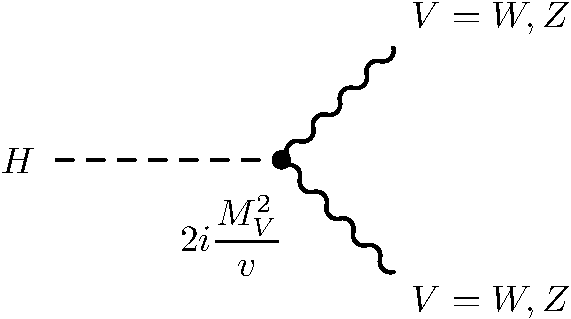
\includegraphics[height=3.5cm]{figures/FD_HVVterm.pdf}
}
\hspace{1cm}
\subfigure[HH-VV interaction]{
\centering
\label{subfig:fd_HHVV}
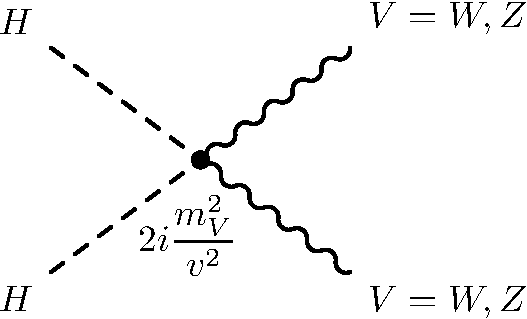
\includegraphics[height=3.5cm]{figures/FD_HHVVterm.pdf}
}
\caption{ Feynman diagrams for (a) H-VV and (b) HH-VV interactions.
}
\label{fig:fd_HVterm}
\end{figure}
The corresponding Feynman diagrams are shown in Fig~\ref{fig:fd_HVterm}. 
Considering additional factorials due to identical particles, the 
vertex factors can be written as $\displaystyle 2i \frac {M_V^2}{v}$ 
and $\displaystyle 2i \frac{M_V^2}{v^2}$ for HVV and HHVV, respectively, 
where V denotes W or Z. 
After SSB, the Higss potential term,  
$\mu^2 \phi^\dagger \phi + \lambda \left( \phi^\dagger \phi \right)^2 $,
in the Lagrangian becomes 
\begin{eqnarray} 
\mathcal{L}_{\textrm{Higgs Potential}}
&=&   
\mu^2 \phi^\dagger \phi + \lambda \left( \phi^\dagger \phi \right)^2 \\ 
&=&   
\frac{\mu^2}{2} ( v + H )^2 + \frac{\lambda}{4} ( v + H )^4 \\ 
%&=&   
%\frac{\mu^2}{2} ( v^2 + H^2 + 2vH ) 
%+ \frac{\lambda}{4} ( v^4 + H^4 + 4v^2H^2 + 2v^2H^2 + 4vH^3 + 4v^3H) \\ 
&=& 
... - \mu^2 H^2 - \frac{\mu^2}{v} H^3  - \frac{\mu^2}{4v^2} H^4 
\end{eqnarray} 
where $H^0$ and $H^1$ terms are ignored in the last line. 
\textcolor{red}{I remember that the first order term does not 
affect the lagrangian, but do not remember the argument.}
From the above eq., the Higgs mass is identified as $\mHi^2 =  -2\mu^2$. %= 2\lambda v^2$.
Rewriting the eq, using this definition, we have  
\begin{eqnarray} 
\mathcal{L}_{\textrm{Higgs Potential}}
&=& 
... - \frac{1}{2} \mHi^2 H^2 - \frac{\mHi^2}{2v} H^3  - \frac{\mHi^2}{8v^2} H^4    
\end{eqnarray}

\begin{figure}[htp]
\centering
\subfigure[HHH interaction]{
\centering
\label{subfig:fd_HHH}
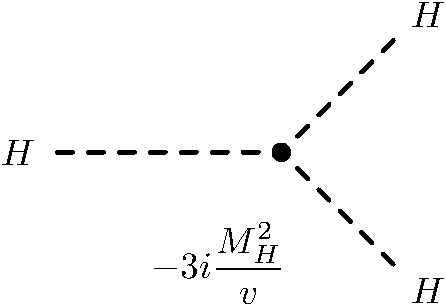
\includegraphics[height=3.5cm]{figures/FD_HHHterm.pdf}
}
\hspace{1cm}
\subfigure[HHHH interaction]{
\centering
\label{subfig:fd_HHHH}
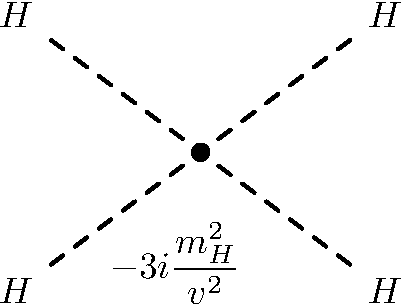
\includegraphics[height=3.5cm]{figures/FD_HHHHterm.pdf}
}
\caption{ Feynman diagrams for (a) HHH and (b) HHHH interactions.
}
\label{fig:fd_Hselfterm}
\end{figure}

The corresponding Feynman diagrams are shown in Fig~\ref{fig:fd_Hselfterm}. 
Now we see that the entire Higgs sector depends on \mHi and $v$.
The $v$ is calculated by $v = \left( \sqrt{2} G_F \right)^{-1/2} = 246~\GeV$  
where $G_F$ is the Fermi contant which is extracted from measurement 
of muon lifetime. 
% G_F meausurement : http://www.sciencedirect.com/science/article/pii/S0168900201012839
Thus, the SM Higgs sector is fully described by \mHi. 
\mHi is a fuction of $\lambda$ and $v$,  $\mHi^2 = 2 \lambda v^2$
and we we do not know the physical meaning of $\lambda$, 
the mass of Higgs boson is not predictable by theory.
It's experimentalist's task to measure \mHi{} and 
complete the Standard Model of particle physics.

The introduced Higgs field had 4 degrees of freedom, $\phi_1, \phi_2, \phi_3$ 
and $\phi_,4$. But, we chose the Higgs field to have only one degree of freedom, $H(x)$.  
Where did the three go? 
By breaking $SU(2)_L \times U(1)_Y$ to $U(1)_{EM}$, the three gauge 
bosons acquired masses. This was done by adding longitudinal components 
to the three bosons. Thus, now we have one physical Higgs field and 
three massive and one massless gauge bosons instead of four unphysical 
Higgs fields and four massless gauge bosons.

The fermions acquire mass by interaction with Higgs field. 
Let's start with leptons whose case is simpler than quarks due to 
absence of right-handed neutrinos, \textit{i.e.} neutrinos are massless.
Below, e means leptons 
We can add SU(2)-invariant terms to the Lagrangian. 
\begin{table}[htb] 
\centering
\begin{tabular}{c c c  }
\hline 
      & $T_3$ & Y \\
\hline \hline 
$\left(  \begin{array}{c} \nu_L \\ e_L \end{array} \right)$      & $\displaystyle  \frac{1}{2} $ & -1 \\
$ \nu_{R}$                                                      & 0 & 0 \\
$ e_R$                                                           & 0 & -2 \\
$\left(  \begin{array}{c} \phi_+  \\ \phi_0 \end{array} \right)$      & $\displaystyle  \frac{1}{2} $ & -1 \\
\hline 
\end{tabular}
\label{tab:su2Qnum}
\caption{$SU(2) \times U(1)$ quantum numbers}
\end{table}
Table \ref{tab:su2Qnum} shows the quantum numbers for $SU(2) \times U(1)$. 
From the table, one can see that the interaction such as 
\begin{eqnarray} 
e_R + \left(  \begin{array}{c} \phi_+  \\ \phi_0 \end{array} \right) 
\rightarrow 
\left(  \begin{array}{c} \nu_L \\ e_L \end{array} \right)
\end{eqnarray} 
conserves quantum numbers. Given the structure of the interaction, 
we specify the strength with $g_e$. Including the hermitian conjugate 
to the Lagrangian, the lepton-Higgs interaction term becomes 
\begin{eqnarray} 
\mathcal{L}_{int, lepton} 
&=& 
-g_e \left[ 
\left(  \begin{array}{cc} \bar{\nu}_L & \bar{e}_L \end{array} \right)
\left(  \begin{array}{c} \phi_+  \\ \phi_0 \end{array} \right) e_R
+ 
\bar{e}_R
\left(  \begin{array}{cc} \bar{\phi}_+  & \bar{\phi}_0 \end{array} \right) 
\left(  \begin{array}{c} \nu_L \\ e_L \end{array} \right)
\right].
\end{eqnarray} 
Using the Higgs field used in SSB 
$\frac{1}{\sqrt{2}} \left(  \begin{array}{c} 0 \\ v + H(x) \end{array} \right)$, 
the Lagrangian is calculated to be 
\begin{eqnarray} 
\mathcal{L}_{int, lepton} 
&=& 
-\frac{g_e v}{\sqrt{2}}\left( \bar{e}_L e_R + \bar{e}_R e_L \right)  
-\frac{g_e H}{\sqrt{2}}\left( \bar{e}_L e_R + \bar{e}_R e_L \right)  
\end{eqnarray} 
Since $\bar{e}e = \bar{e}(P_L^2+P_R^2)e = \bar{e}_L e_R + \bar{e}_R e_L$ where
$P_L$ and $P_R$ are projection operators, the first term 
$\displaystyle -\frac{g_e v}{\sqrt{2}} \bar{e}e$ corresponds to the mass term for lepton. 
Thus, the mass is identified to be 
\begin{eqnarray} 
m_e = \frac{g_e v}{\sqrt{2}}.
\end{eqnarray} 
Rewriting the Lagrangian in terms of $m_e$ instead of an arbitary $g_e$, we get 
\begin{eqnarray} 
\mathcal{L}_{int} 
&=& 
- m_e \bar{e}e  -\frac{m_e}{v} \bar{e}e H. 
\end{eqnarray} 
Since there isn't a physical motivation for $g_e$, $m_e$ is not calculable 
by theory, but needs to be experimentally determined. The second term 
corresponds to lepton-Higgs interaction. The size of the interaction 
is proportional to the mass of lepton. Thus, light quarks have very 
weak couplings to Higgs fields. For example, electron has 
$\displaystyle \frac{m_e}{v} = \frac{0.5~\MeV}{246~\GeV} \sim \mathcal{O}\left(10^{-6}\right)$
and muon has $\displaystyle \frac{106~\MeV}{246~\GeV} \sim \mathcal{O}\left(10^{-3}\right)$.

The case for quarks is more complicated due to presence of right-handed up-type 
quarks opposite to lepton case. In order to generate masses for up-type 
quarks, we need a new Higgs doublet 
\begin{eqnarray} 
\phi_c 
= i \sigma_2 \phi^* 
=  \left(  \begin{array}{c} \phi_0^* \\ -\phi_- \end{array} \right) 
=  \frac{1}{\sqrt{2}} \left(  \begin{array}{c} v + H(x) \\ 0 \end{array} \right). 
\end{eqnarray} 
The new Higgs field is invariant under $SU(2)$ transformation and has Y = -1. 
\begin{eqnarray} 
\mathcal{L}_{int, quark} 
&=& 
-g_{d} \left[ 
\left(  \begin{array}{cc} \bar{u}_L & \bar{d}_L \end{array} \right)
\left(  \begin{array}{c} \phi_+  \\ \phi_0 \end{array} \right) d_R  \right]
-g_{u} \left[ 
\left(  \begin{array}{cc} \bar{u}_L & \bar{d}_L \end{array} \right)
\left(  \begin{array}{c} \phi_0^*  \\ -\phi_+ \end{array} \right) u_R  \right] 
+ h.c. \\
%&=& 
%-\frac{g_d v}{\sqrt{2}}\left( \bar{d}_L d_R + \bar{d}_R d_L \right)  
%-\frac{g_d H}{\sqrt{2}}\left( \bar{d}_L d_R + \bar{d}_R d_L \right)  
%-\frac{g_u v}{\sqrt{2}}\left( \bar{u}_L u_R + \bar{u}_R u_L \right)  
%-\frac{g_u H}{\sqrt{2}}\left( \bar{u}_L u_R + \bar{u}_R u_L \right) \\
&=&  
-\frac{g_d v}{\sqrt{2}} \bar{d}d - \frac{g_d H}{\sqrt{2}} \bar{d}d  
-\frac{g_u v}{\sqrt{2}} \bar{u}u - \frac{g_u H}{\sqrt{2}} \bar{u}u \\
&=&  
- m_d \bar{d}d  -\frac{m_d}{v} \bar{d}d H
- m_u \bar{u}u  -\frac{m_u}{v} \bar{u}u H
\end{eqnarray} 
where 
\begin{eqnarray} 
m_d = \frac{g_d v}{\sqrt{2}} \quad \textrm{ and } \quad   
m_u = \frac{g_u v}{\sqrt{2}}
\end{eqnarray} 
is used as the lepton case. The strength of interaction depends on the 
fermion mass, $m_f / v$. 
\begin{figure}[htp]
\centering
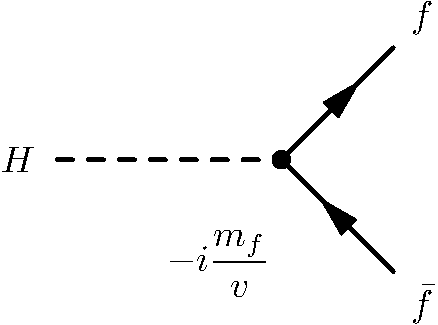
\includegraphics[height=3.5cm]{figures/FD_HFFterm.pdf}
\caption{ Feynman diagram for Hff interaction.}
\label{fig:fd_HFFterm}
\end{figure}

Fig. \ref{fig:fd_HFFterm} shows Feynman diagram for Higgs - fermion interaction.    





%%%%%%%%%%%%%%%%%%%%%%%%%%%%%%%%%%%%%%%%%%%%%%%%%%%%%%%%%%%%%%%%
\section{Production and Decay of Higgs Boson}


\subsection{Production of Higgs Boson}
Standard model Higgs boson is generated by 4 major processes, 
gluon-gluon fusion (ggH : $gg \rightarrow H$), 
vector boson fusion (qqH : $q\bar{q}\rightarrow H$),
associated production with vector bosons (VH : $q\bar{q}\rightarrow VH$), and 
associated production with heavy quarks(QQH : $q\bar{q}\rightarrow Q\bar{Q}H$). 
Figure X.X shows the Feynman diagrams corresponding those mechanisms.
Since H does not couple to gluon in ggH process it is produced via a top loop.
At LHC ggH has the largest production rate due to PDF and 
the heaviness of top quark. 
\begin{figure*}[t]
\centering
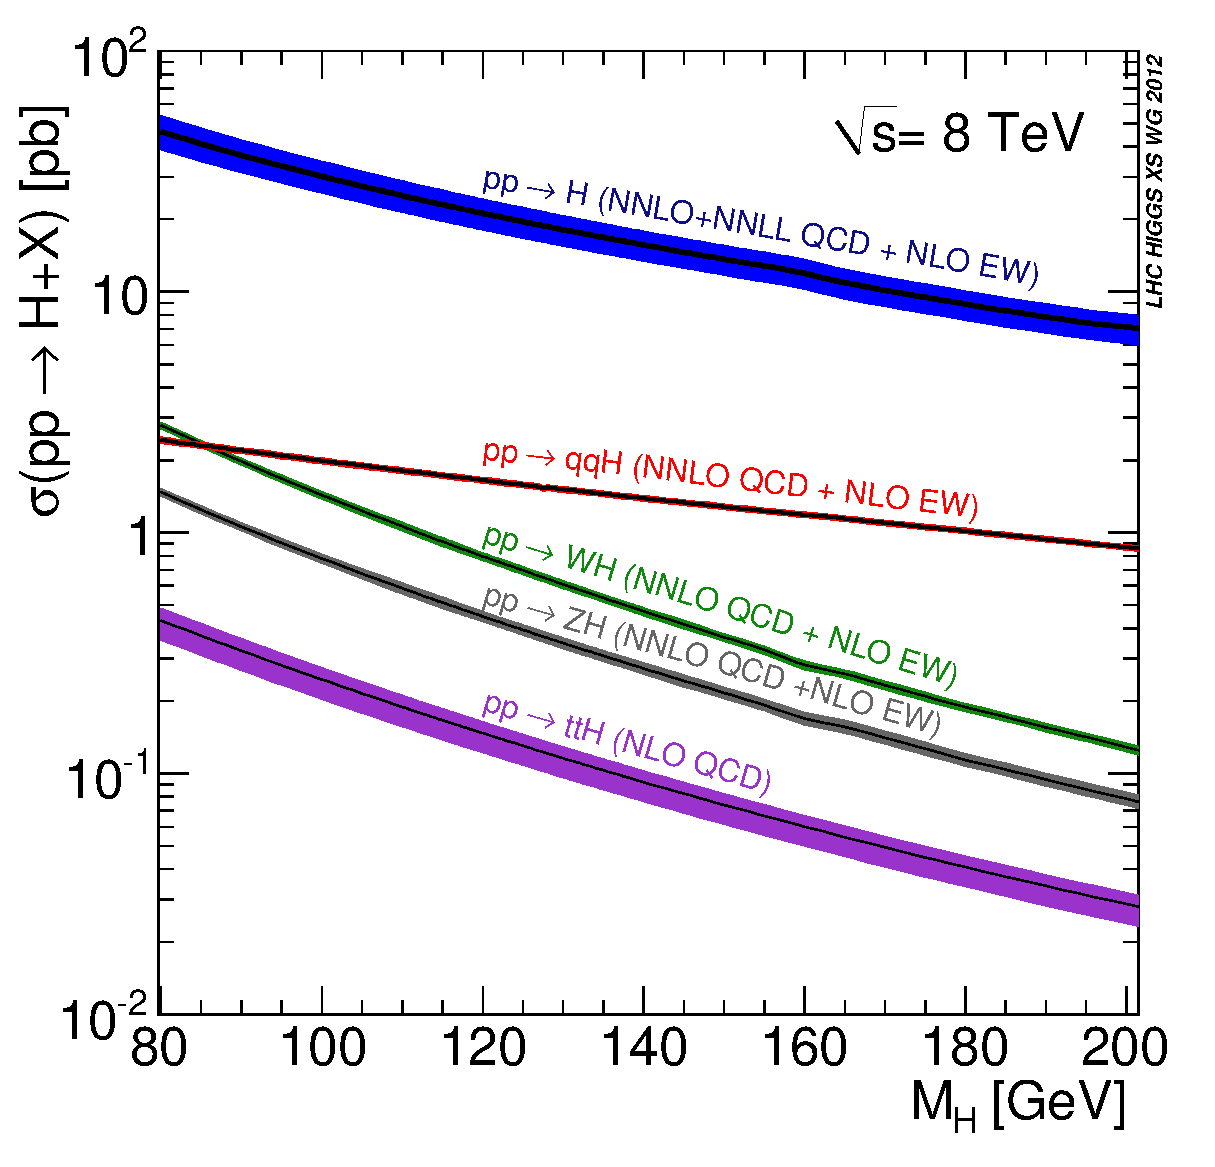
\includegraphics[width=0.8\textwidth]{figures/Higgs_XS_8TeV_LM200.eps}
\caption{ Standard model Higgs production cross sections 
as a function of \mHi{} at $\sqrt{s}=8TeV$ for each 
production mode \cite{Dittmaier:2012vm}. The ggF and VBF processes are 
calculated in complex-pole-scheme (CPS), while other WH/ZH and ttH processes 
are calculated in zero-width-approximation (ZWA). }
\label{fig:Higgs_XS_8TeV_LM200}
\end{figure*}

At hadron collider the hadronic cross section($\sigma$) is calculated with 
parton-level cross-section ($\hat{\sigma}$) convoluted with PDF, 
\begin{eqnarray} 
\sigma (pp \rightarrow H+X) 
= 
\sum_{i,j} \int dx_1 dx_2 f_i(x_1) f_j(x_2) 
\hat{\sigma} \left( ij \rightarrow H+X \right)
\end{eqnarray} 
where i and j are colliding partons, 
$x_1$ and $x_2$ are longitudinal momentum fractions carried by i and j. 
Each component in the equation is subject to the following uncertainties.
The partonic cross section is calculated at given
a renormalizaion scale $\mu_R$ and a factorization scale $\mu_F$. 
Due to possible uncalculated higher-order QCD radiative corrections,
the uncertainty is estimated by varying the scales around 
the central values. In the de Florian and Grazzini (dFG) 
calculation [ref], the central values are chosen to be $\mu_0 = \mHi$. 
The scales $\mu_R$ and $\mu_F$ are varied are in the range 
$\displaystyle \frac{1}{2}\mu_0 < \mu_F, \mu_R < 2\mu_0$ 
with a constraint $\displaystyle \frac{1}{2} < \frac{\mu_F}{\mu_R} < 2$. 
PDF is obtained by fitting on data measured in deep-inelastic scattering, 
Drell-Yan, and jet production from a wide variety of different experiments. 
The accuracy on those data can introduce uncertainty on PDF calculation. 
In addition, strong coupling constant $\alpha_s$ is used in DGLAP evolution [ref] 
to the higher $Q^2$ region. Thus, its uncertainty also contributes to 
the total cross section. There are other uncertainties due to 
the EW corrections, the different choice of top and bottom quark masses, 
and the use of large-$m_T$ method. But, the effect to the 
hadronic cross section is less than a few percent \cite{Dittmaier:2012vm}
for ggF.

Figure \ref{fig:Higgs_XS_8TeV_LM200} shows the hadronic cross sections 
as a function of \mHi{} for SM Higgs production and uncertainty 
in different production modes. The ggF and VBF cross sections 
are based on complex-pole-scheme (CPS), while VH and ttH ones 
are based on zero-width-approximation (ZWA). 
\begin{table}[htb]
\centering
\begin{tabular}{c c c  }
\hline
process     & QCD   & EW \\
\hline \hline 
$ pp \rightarrow H$         & NNLO  & NLO \\
$ pp \rightarrow qqH$       & NNLO  & NLO \\
$ pp \rightarrow WH$        & NNLO  & NLO \\
$ pp \rightarrow ZH$        & NNLO  & NLO \\
$ pp \rightarrow ttH$       & NLO   &     \\
\hline 
\end{tabular}
\label{tab:Higgs_XS_8TeV_order}
\caption{The order of QCD and EW calculations.}
\end{table}
The order of QCD and EW calculations are summarized in Table 
\ref{tab:Higgs_XS_8TeV_order}. The uncertainty is linear combination 
of uncertainties from QCD scale varitaion and PDF+$\alpha_S$.
At $\mHi=125~\GeV$ ggH contributes $\sim 87 \%$ to the total cross section.


%The PDF and parton-level cross section depend on the 
%renormalizaion scale $\mu_R$ because they contain ultraviolet divergences 
%to be subtacted through a renormalization procedure. [ref] 
%In addition PDF is calculated with a factorization scale $\mu_F$.

%%%
\subsection{Decay of Higgs Boson}
The interaction term in the Lagrangian shows that the Higgs can 
couple to a pair of weak bosons($VV$). Thus, Higgs decays into $W^+W^-$ and $ZZ$.
Depending on the mass of Higgs, one or two of the bosons can be off-shell. 
Thus we consider three cases where both of them are on-shell$(VV)$, 
one is on-shell and the other is off-shell$(VV^*)$, 
and both of them are off-shell$(V^*V^*)$. 
\begin{itemize} 
%
\item  Both bosons are on-shell($ H \rightarrow VV$) [ref] : 
\begin{eqnarray} 
\Gamma \left( H \rightarrow VV \right) 
= 
\frac{G_F \mHi^3}{16\sqrt{2\pi}} \delta_V \sqrt{1-4\epsilon^2} 
\left( 1 - 4\epsilon^2 - 12\epsilon^4 \right)
\end{eqnarray} 
where $\displaystyle \epsilon = \frac{M_V}{\mHi}$ and $\delta_W=2$ and $\delta_Z=1$.
The ratio of londitudinal polarization is given by \cite{PhysRevD.49.79}
\begin{eqnarray} 
R_L 
= 
\frac{\Gamma_L}{\Gamma_T + \Gamma_L}    
= 
\frac{1 - 4\epsilon^2 - 4\epsilon^4}{1 - 4\epsilon^2 - 12\epsilon^4} 
\xrightarrow{\epsilon \rightarrow 0}{} 1
\end{eqnarray} 
Thus, vector bosons are longitudinally polarized at high \mHi{} ($\epsilon \rightarrow 0$). 
At the production threshold, $\displaystyle \mHi = 2M_V \rightarrow \epsilon = \frac{1}{2}$, 
$R_L$ is 2 which means that longitudinal and transverse polarizations are equally populated. 
In addition, the decay width to WW is reduced to 
\begin{eqnarray} 
\Gamma \left( H \rightarrow WW \right)
&\rightarrow&
\frac{G_F \mHi^3}{16\sqrt{2\pi}} \times 2 \\
&=&  
2 \frac{ 1.16637 \times 10^{-5}~\GeV^{-2} \mHi^3}{16\sqrt{2\pi}} \\
&\approx&
0.33 \mHi \times \frac{\mHi^2}{TeV^2} (TeV).   
\end{eqnarray} 
For example, at $\mHi=1TeV$, decay width for WW is 0.33 TeV.
Practically t is hard to claim a Higgs resonance at high mass regions.  
%
\item  one is on-shell and the other is off-shell 
       ($ H \rightarrow VV^* \rightarrow Vf\bar{f}$) where $f$ does not include top quark [ref] : 
\begin{eqnarray} 
\Gamma \left( H \rightarrow VV^* \right) 
=
\frac{3G_F^2 M_v^4}{16\pi^3} \mHi \delta_V' R(\epsilon)
\end{eqnarray} 
where $\delta_W'=1$, $\displaystyle \delta_Z'=\frac{7}{12}-\frac{10}{9}\sin^2\theta_W 
+ \frac{40}{9}\sin^4\theta_W$, and 
\begin{eqnarray}   
\begin{array}{ccc} \multicolumn{2}{c}{\displaystyle 
Rf(\epsilon) = \frac{3(1-8\epsilon^2+20\epsilon^4)}{(4\epsilon^2-1)^{1/2}} 
                \arccos \left( \frac{3\epsilon^2-1}{2\epsilon^3} \right)  
} & \\ & \multicolumn{2}{c}{\hspace{1.5cm} \displaystyle
- (1-\epsilon^2)\left( \frac{47}{2}\epsilon^2 - \frac{13}{2} + \frac{1}{\epsilon^2} \right)  
- 3(1-6\epsilon^2+4\epsilon^4) \ln \epsilon
} \end{array}      
\end{eqnarray} 
\end{itemize} 
The ratio of londitudinal polarization is given \cite{PhysRevD.49.79} by 
\begin{eqnarray} 
R_L 
=
\frac{\Gamma_L}{\Gamma_T + \Gamma_L}    
= 
\frac{R_L(\epsilon)}{R(\epsilon)}  
\end{eqnarray} 
where $R_L$ is \cite{PhysRevD.49.79} 
\begin{eqnarray} 
\begin{array}{ccc} \multicolumn{2}{c}{\displaystyle 
R_L(\epsilon) = \frac{3(1-16\epsilon^2+20\epsilon^4)}{(4\epsilon^2-1)^{1/2}} 
                \arccos \left( \frac{3\epsilon^2-1}{2\epsilon^3} \right)  
} & \\ & \multicolumn{2}{c}{\hspace{1.5cm} \displaystyle
- (1-\epsilon^2)\left( \frac{15}{2}\epsilon^2 - \frac{13}{2} + \frac{1}{\epsilon^2} \right)  
- (3-10\epsilon^2+4\epsilon^4) \ln \epsilon.
} \end{array}      
\end{eqnarray} 

\begin{figure*}[t]
\centering
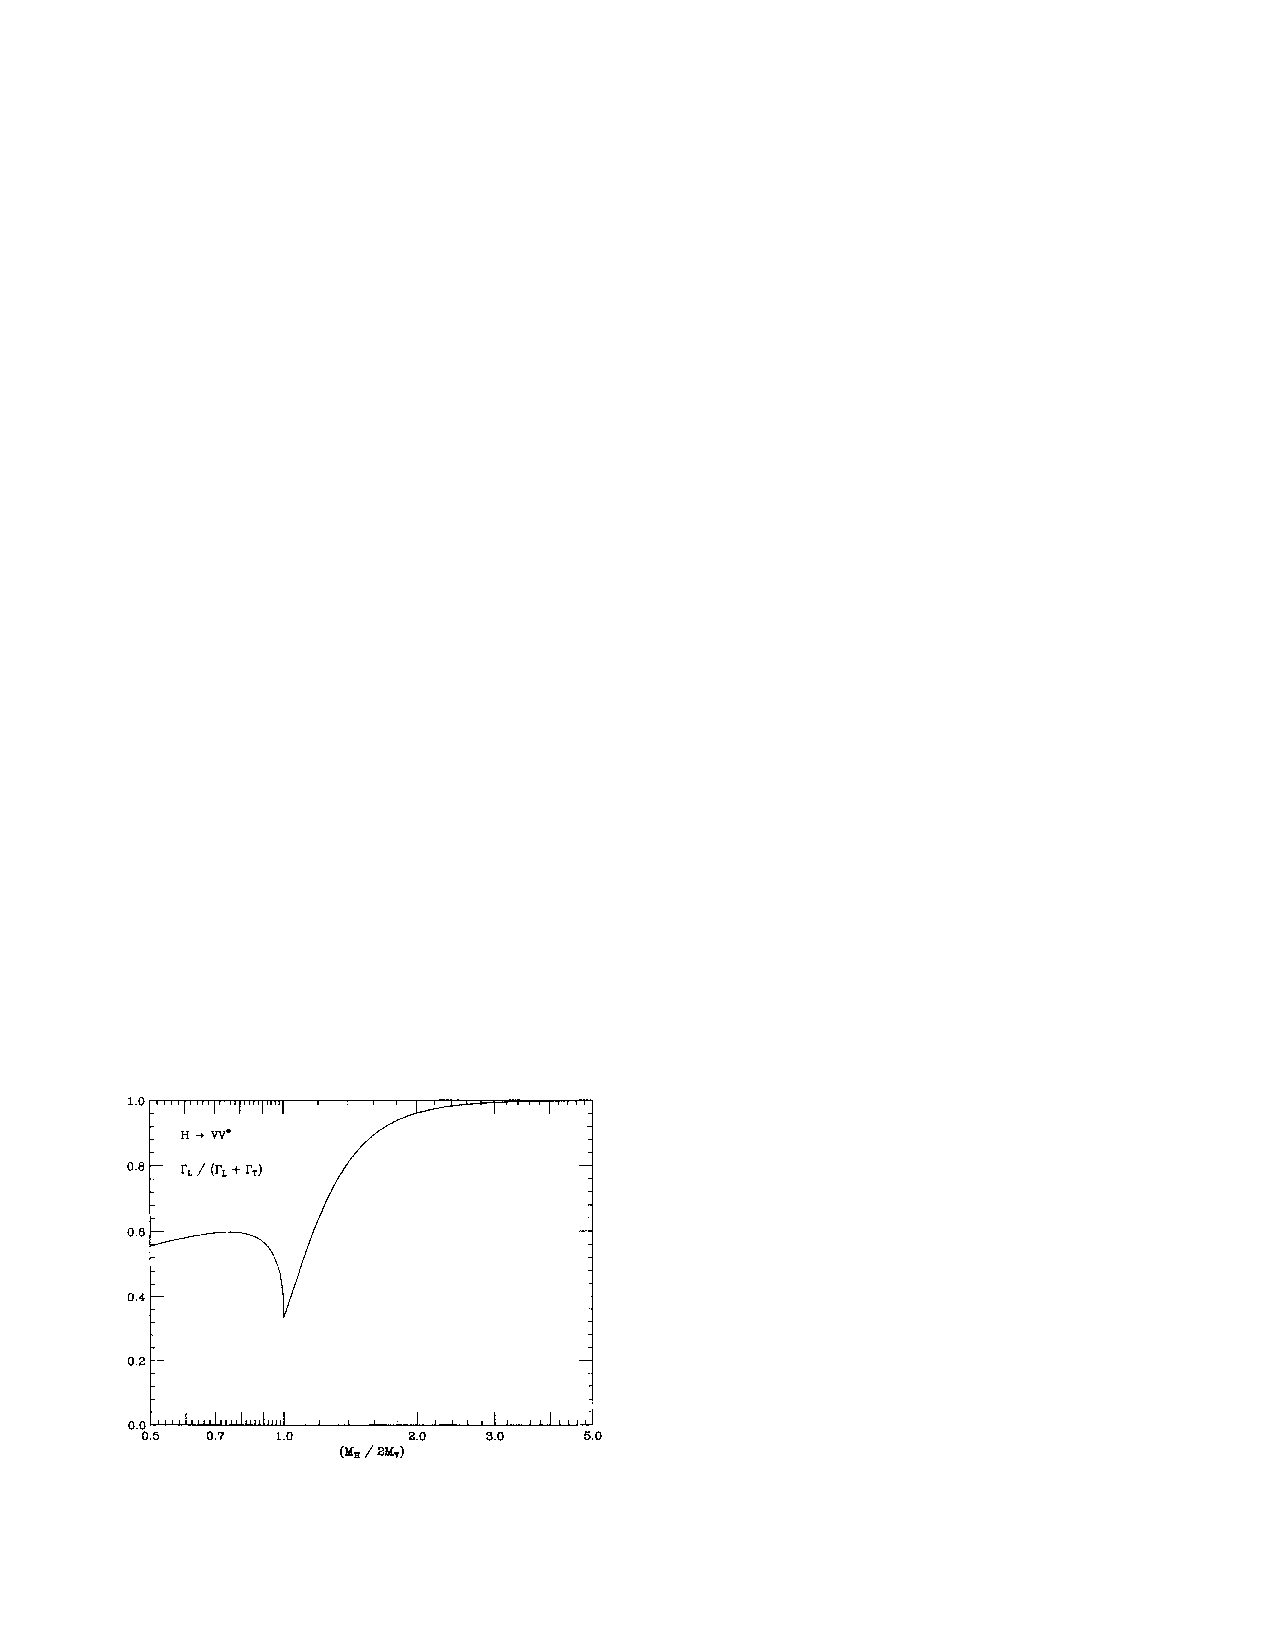
\includegraphics[width=0.6\textwidth]{figures/HVV_polarization_ratio.pdf}
\caption{The ratio of longitudinal polarization of vector bosons 
as a function of $\frac{\mHi}{2M_V}$ \cite{PhysRevD.49.79} }
\label{fig:HVV_polarization_ratio}
\end{figure*}
Figure \ref{fig:HVV_polarization_ratio} shows the ratio of longitudinally 
polarized vector bosons as a function of $\displaystyle \frac{\mHi}{2M_V}$
(=$\displaystyle \frac{\epsilon}{2}$). 
The ratio changes as \mHi{} changes. Thus, we expect event kinematics differs 
with different \mHi{} hypotheses. This is important when we define signal 
regions optimized at a given \mHi{} hypothesis.  
\textcolor{red}{mention $\Delta\phi_{ll}$ here? What does it mean that 
Vs are transervely polarized? (schemetically)}

\begin{figure*}[t]
\centering
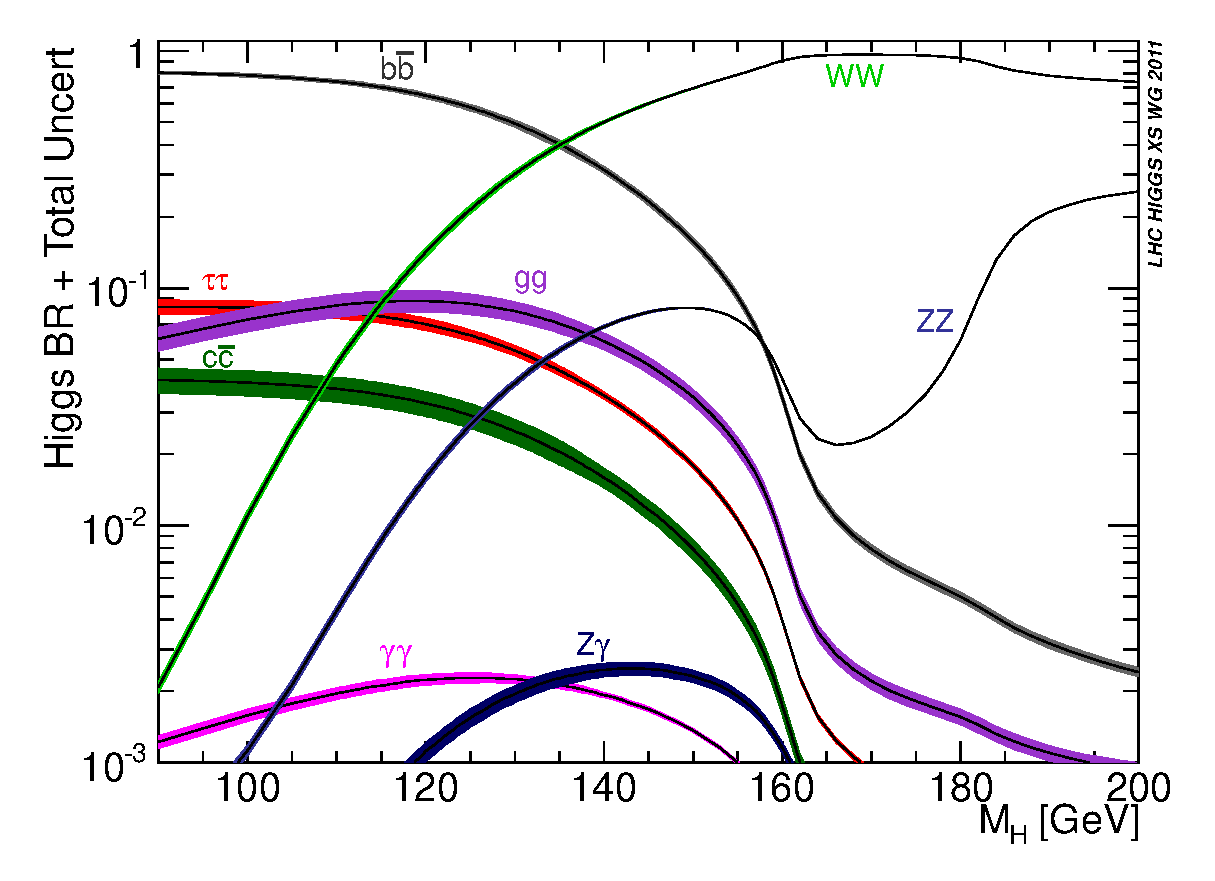
\includegraphics[width=0.45\textwidth]{figures/YRHXS2_BR_Fig1.eps}
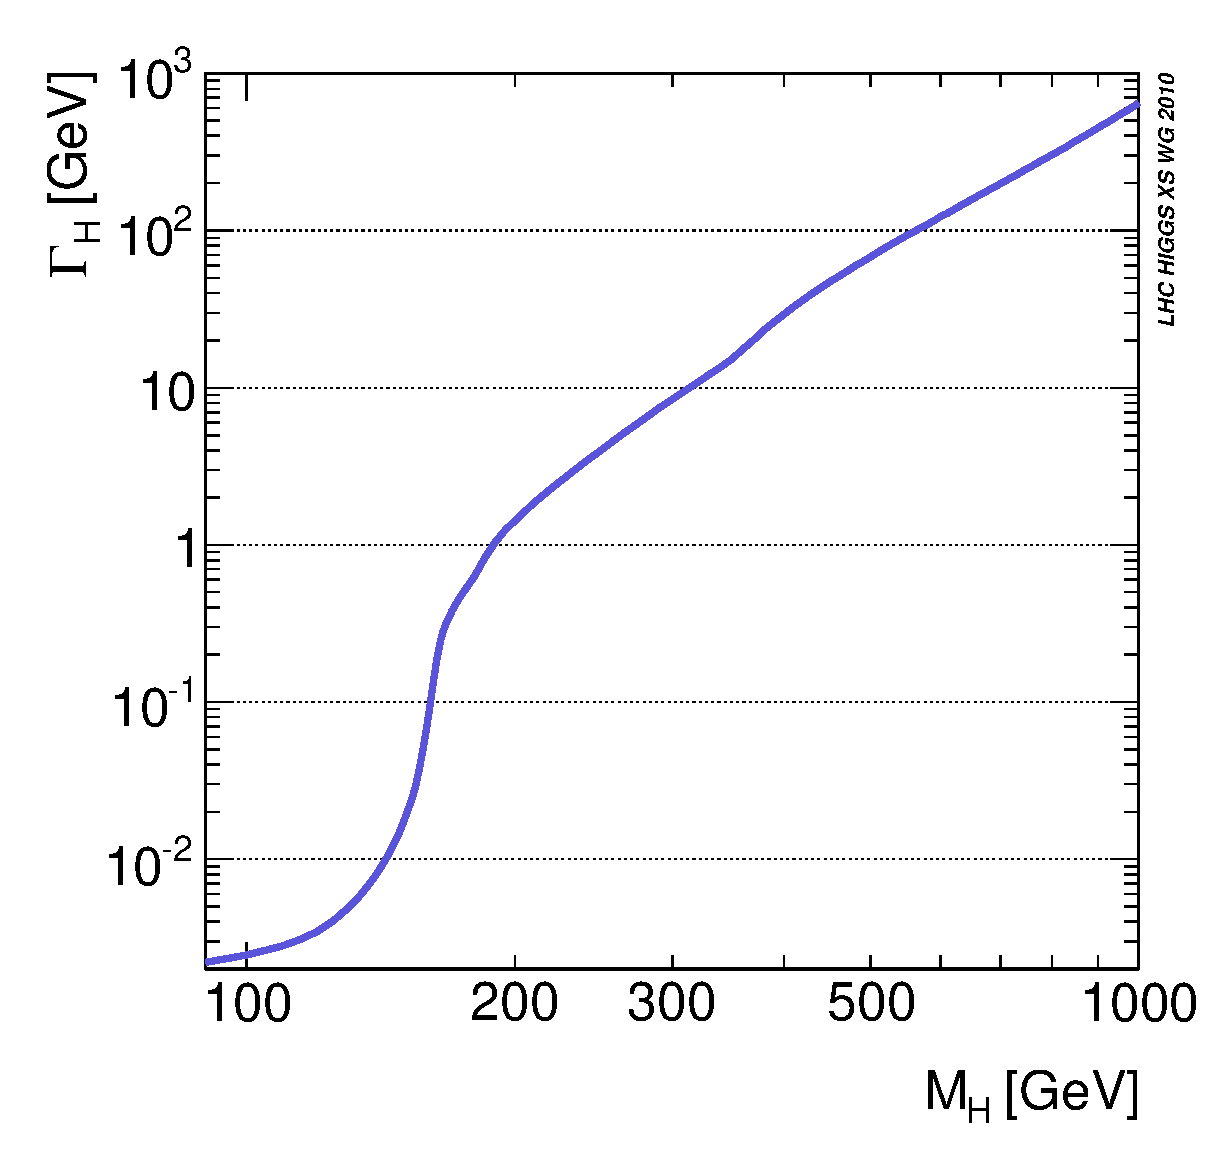
\includegraphics[width=0.45\textwidth]{figures/YRHXS_BR_fig2}
\caption{Standard Model Higgs boson decay branching ratios at low \mHi(left) 
and total width (right).}
\label{fig:YRHXS2_BR_Fig1}
\end{figure*}
Figure \ref{fig:YRHXS2_BR_Fig1} shows the branching ratios of Standard 
Model Higgs boson and its total decay width. \textcolor{red}{Top and bottom quarks are 
included in the calculation. Uncertainties are from ...} 

\begin{figure*}[t]
\centering
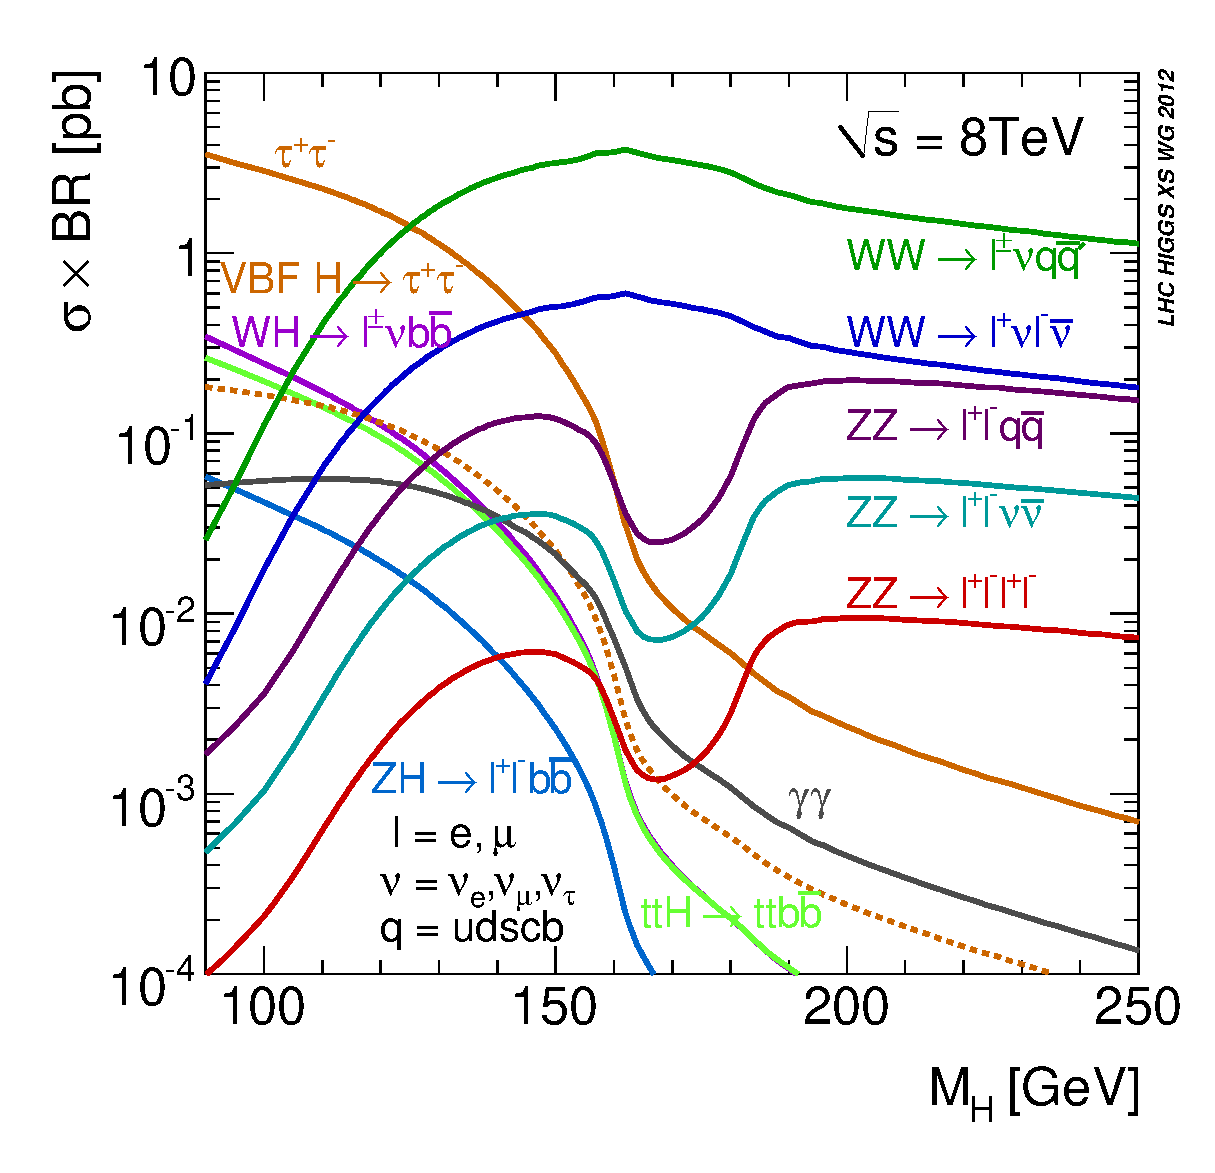
\includegraphics[width=0.6\textwidth]{figures/XSBR_8TeV_SM_LM.eps}
\caption{$\sigma \times BR$ at low \mHi.}
\label{fig:XSBR_8TeV_SM_LM}
\end{figure*}

\begin{table}[htb]
\centering
\begin{tabular}{c c c c c}
\hline 
        & $H \rightarrow WW \rightarrow 2l2\nu$   & $H \rightarrow ZZ\rightarrow 4l$ 
        & $H \rightarrow\gamma\gamma$ & $H \rightarrow\tau\tau$\\ 
\hline \hline 
$\sigma \times BR (pb)$  
        & $2.24\times10^{-1}$ &  $2.79\times10^{-3}$ & $5.09\times10^{-2}$ & $1.41$ \\ 
$N_{expected}$ in $\mathcal{L}_{int} = 20 fb^{-1}$ 
        & 4480 &  56 & 1018 & 28200 \\ 
\hline 
\end{tabular}
\label{tab:XSBR_8TeV_SM_125}
\caption{$\sigma \times BR$ at $\mHi=125~\GeV$ for most sensitive channels 
and the expected number of events in $\mathcal{L}_{int} = 20 fb^{-1}$.
l means electrons or muons.}
\end{table}
Figure \ref{fig:XSBR_8TeV_SM_LM} shows $\sigma \times BR$ at low \mHi.
Table \ref{tab:XSBR_8TeV_SM_125} shows the corrsponding numbers at $\mHi=125~\GeV$
for most sensitive channels and the expected number of events 
($\sigma \times BR \times \mathcal{L}_{int}$) at $\mathcal{L}_{int} = 20 fb^{-1}$.
WW is .. 


%%%%%%%%%%%%%%%%%%%%%%%%%%%%%%%%%%%%%%%%%%%%%%%%%%%%%%%%%%%%%%%%
\section{Limits on Higgs Boson Mass} 

\subsection{Theoretical Limits} 

\subsubsection{Unitarity : $W_L^+W_L^- \rightarrow W_L^+W_L^-$}

\subsubsection{Triviality and Stability bounds}
The variation of $\lambda$ is described by Renormalization Group Equation (RGE).
When we consider one-loop radiation correction to the Higgs boson quartic coupling
(Fig \ref{fig:FD_triviality}), the corresponding RGE is given by \cite{Djouadi20081} 
\begin{eqnarray}
\frac{d}{dQ^2} \lambda (Q^2) = \frac{3}{4\pi^2} \lambda^2(Q^2) 
+ \textrm{higher orders}
\end{eqnarray} 
The solution to this equation is given by 
\begin{eqnarray} 
\displaystyle  
\lambda(Q^2) 
= \frac{\lambda(v^2)}
       {\left[ 1 - \frac{3}{4\pi^2} \lambda(v^2) \log{\frac{Q^2}{v^2}}\right] } 
\end{eqnarray} 
where EWSB scale $Q_0 = v$ is used as a energy reference frame. 



\subsubsection{Fine tuning}

\subsection{Experimental Limits} 
* EWK precision fit 


%%%%%%%%%%%%%%%%%%%%%%%%%%%%%%%%%%%%%%%%%%%%%%%%%%%%%%%%%%%%%%%%
\section{Alternative Models} 
minimally coupled graviton-like Spin2
